\documentclass[11pt,a4paper]{article}
% Shared preamble for the template and the worked example.
\usepackage[a4paper,margin=22mm,top=19mm,bottom=22mm]{geometry}
\usepackage{amsmath,amssymb}
\usepackage{array,booktabs,tabularx}
\usepackage{graphicx,float,caption}
\usepackage{xcolor}
\usepackage{microtype}
\usepackage{hyperref}

\definecolor{ReportInk}{HTML}{193548}
\definecolor{ReportMuted}{HTML}{496071}
\hypersetup{colorlinks=true,linkcolor=ReportInk,citecolor=ReportInk,urlcolor=ReportInk}
\captionsetup{font=small,labelfont=bf,labelsep=period,skip=5pt}
\setlength{\parindent}{0pt}
\setlength{\parskip}{3pt plus 1pt}
\setlength{\textfloatsep}{12pt plus 2pt minus 3pt}
\setlength{\intextsep}{6pt plus 2pt minus 2pt}
\setlength{\emergencystretch}{1em}
\renewcommand{\arraystretch}{1.12}
\raggedbottom
\clubpenalty=10000
\widowpenalty=10000

\makeatletter
\renewcommand\section{\@startsection{section}{1}{\z@}%
  {-11pt plus -2pt minus -1pt}{5pt plus 1pt}{\normalfont\large\bfseries}}
\renewcommand\subsection{\@startsection{subsection}{2}{\z@}%
  {-8pt plus -2pt minus -1pt}{4pt plus 1pt}{\normalfont\normalsize\bfseries}}
\renewcommand\paragraph{\@startsection{paragraph}{4}{\z@}%
  {6pt plus 1pt}{-0.65em}{\normalfont\normalsize\bfseries}}
\makeatother
\AtBeginDocument{%
  \setlength{\abovedisplayskip}{6pt plus 2pt minus 2pt}%
  \setlength{\belowdisplayskip}{6pt plus 2pt minus 2pt}}

\newcommand{\reporttitle}[2]{%
  {\small\bfseries\color{ReportMuted} MATH11007\enspace\textbar\enspace
  Methodology, Modelling and Consulting Skills\par}
  \vspace{5pt}
  {\LARGE\bfseries\color{ReportInk}#1\par}
  \vspace{4pt}
  {\small #2\par}
  \vspace{6pt}
  {\color{ReportInk}\hrule height 0.5pt}
  \vspace{5pt}}
\newcommand{\guidance}[1]{\textit{\color{ReportMuted}[#1]}}
\newcommand{\gbp}{\pounds}
\newcommand{\hydrogen}{\ensuremath{\mathrm{H}_2}}
\newcolumntype{Y}{>{\raggedright\arraybackslash}X}
\newcolumntype{M}[1]{>{\raggedright\arraybackslash}m{#1}}
\newcommand{\negval}[1]{\ensuremath{-\mathrm{#1}}}
% The worked example may break at topic boundaries. The group report reflows.
\newcommand{\samplebreak}{}

\hypersetup{pdftitle={Investment in Storage and Hydrogen}}
\renewcommand{\samplebreak}{\newpage}

\begin{document}
\reporttitle{Investment in Storage and Hydrogen}
  {Group 15\quad\textbar\quad Technical report, Tier 1\quad\textbar\quad 2026/27}

\section*{Executive summary}
Under economic dispatch in 2023, one 20~MW electrolyser and no battery
add \gbp 8.57m per year at a netback of \gbp 7.799/kg and an offtake cap
of 10~t/day. Daily electricity priority selects zero investment. The
20~MW plant captures 13.92~GWh of 549.94~GWh of physical surplus.
The rest of its electricity input, 157.92~GWh, would otherwise have
been sold. The economic case rests on the value of that diversion and
the buyer's terms.

\section{Decision context and data}\label{sec:data}
The constructed system combines the supplied generation portfolio with the
simulated wind farm \cite{brief}. Existing generation is fixed. Demand caps
electricity sales, imports are excluded and unused output has zero value.
Daily mean MW is multiplied by 24~h. We use 2023 to choose capacity.

\begin{table}[H]
  \centering\small
  \caption{Input checks and repairs. The audit records replacements and
  flags estimates. Date counts can overlap \cite{repair}.}
  \label{tab:repairs}
  \begin{tabularx}{\linewidth}{@{}M{0.23\linewidth}Y@{}}
    \toprule
    Check & Treatment \\
    \midrule
    Calendar and totals & Align five series to 2,452 UTC days (January 2020 to
      17 September 2026). Reconcile generation by fuel to total generation. \\
    Midnight snapshots & Rebuild full days for 7 generation, 350 demand and
      346 price endpoints. \\
    Price aggregation & Volume-weight active providers within periods, then
      average across the day. Rebase to 2020 pounds with monthly CPI \cite{cpi}. \\
    Gaps and anomalous zeros & Use observed intervals where available, then
      flag interpolated or proxy values. A strict-quality sensitivity retains
      280 days in 2023. \\
    \bottomrule
  \end{tabularx}
\end{table}

\begin{figure}[H]
  \centering
  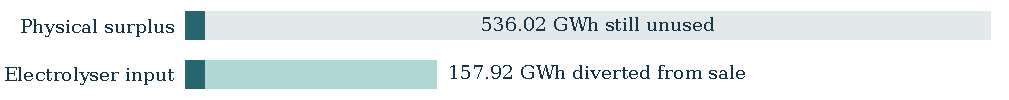
\includegraphics[width=\linewidth]{figures/energy-balance.pdf}
  \caption{2023 physical surplus and electrolyser input under A.
    The dark segment in each bar is the same 13.92~GWh of captured surplus.}
  \label{fig:surplus}
\end{figure}

\section{Tier 1. Flexibility investment}\label{sec:tier1}
\subsection{Technology and economic assumptions}
The brief's EUR~288,000/MWh converts to \gbp 256,235/MWh at the 2020
exchange rate \cite{brief,basis}. For its \gbp 9.50/kg support benchmark,
we use the published 2012 basis: \gbp 175/MWh times 39.4~kWh/kg, then
rebase by CPI to \gbp 7.799/kg \cite{har,cpi,basis}. The 10~t/day offtake
cap is a buyer scenario.

\begin{table}[H]
  \centering\small
  \caption{Equipment and finance assumptions. All model prices are in 2020 pounds.}
  \label{tab:assumptions}
  \begin{tabularx}{\linewidth}{@{}M{0.15\linewidth}Y@{}}
    \toprule
    Input & Assumption \\
    \midrule
    Battery & 1.5~MW / 3~MWh per module. 20--80\% state of charge, 90\% round-trip
      efficiency, \gbp 14,862/MW-year fixed cost, 15-year life \cite{brief,dea}. \\
    Electrolyser & 20~MW per module, 20--100\% online load and 55.9~kWh/kg.
      Installed cost \gbp 29.21m per module (IEA midpoint). UK cost proxies
      give \gbp 0.517m fixed cost per year and \gbp 9.79m renewals in years
      11 and 22 of a 30-year life \cite{iea,beis,basis}. \\
    Finance & 5\% real discount rate. Hydrogen netback is after non-power variable costs. \\
    \bottomrule
  \end{tabularx}
\end{table}

\samplebreak
\subsection{Mixed-integer formulation}\label{sec:formulation}
For days \(t\in\mathcal T\), supply \(G_t\) and demand \(D_t\) are in MWh.
The wholesale price \(p_t\) is in \gbp/MWh, hydrogen netback \(v\) is in
\gbp/kg, and \(L\) limits hydrogen sales in kg/day. The decision variables
\(q_t,c_t,r_t,h_t,u_t\) are direct sale, charge, discharge, electrolyser
input and unused generation in MWh. Installed module counts are \(b,n\)
for the battery and electrolyser, and \(z_t\) counts online electrolyser
modules. The model uses \(\kappa=0.0559\)~MWh/kg and equivalent annual
costs \(a_B,a_H\). The sample represents \(Y\) years, with \(Y=1\) for
a full calendar year and \(Y=280/365\) in the strict-quality case.

\begin{subequations}\label{eq:tier1-model}
\begin{align}
  \max\quad & \frac{1}{Y}\sum_{t\in\mathcal T}
    \left[p_t(q_t+r_t)+v\frac{h_t}{\kappa}\right]-a_B b-a_H n,
      \label{eq:objective}\\
  \text{subject to}\quad
    & q_t+c_t+h_t+u_t=G_t,\qquad q_t+r_t\le D_t,
      \label{eq:balance}\\
    & c_t\le E_Bb/\eta,\qquad r_t\le \eta E_B b,\qquad
      \sum_{t\in\mathcal T}r_t=\eta^2\sum_{t\in\mathcal T}c_t,
      \label{eq:battery}\\
    & E_H^{\min}z_t\le h_t\le E_H^{\max}z_t,\qquad
      h_t/\kappa\le L,\qquad z_t\le n,
      \label{eq:electrolyser}\\
    & q_t,c_t,r_t,h_t,u_t\ge0,\qquad b,n,z_t\in\mathbb Z_{\ge0}.
      \label{eq:domain}
\end{align}
\end{subequations}

The day-indexed constraints apply for all \(t\).
Equation~\eqref{eq:balance} allocates supply and limits electricity sales.
Equation~\eqref{eq:battery} allows one usable battery window per day and
balances energy over the year, with \(E_B=1.8\)~MWh and \(\eta=\sqrt{0.90}\).
In \eqref{eq:electrolyser}, \(E_H^{\min}=96\) and \(E_H^{\max}=480\)~MWh
bound daily input per online module and \(L\) caps output.
Policy A uses economic dispatch. Policy B additionally fixes
\(q_t=\min\{G_t,D_t\}\). B therefore incurs negative sales revenue when
the price is negative (two days in 2020, none in 2023).

For technology \(j\in\{B,H\}\), equivalent annual cost is
\begin{equation}
  a_j=F_j+\frac{i}{1-(1+i)^{-N_j}}
    \left(K_j+\sum_{k\in\mathcal R_j}\frac{C_{jk}}{(1+i)^k}\right),
  \label{eq:annual-cost}
\end{equation}
where \(i\) is the real discount rate, \(N_j\) the service life, \(F_j\)
annual fixed cost, \(K_j\) upfront cost including commissioning and \(C_{jk}\)
the cost of a renewal in year \(k\in\mathcal R_j\). Gains subtract the
zero-investment objective under the same policy.

\subsection{Portfolio results and matched operating rule}
The simple rule sells electricity first, then produces hydrogen from the
remainder subject to loading and offtake limits. With 20~MW it yields
\negval{}\gbp 1.07m/year. Economic dispatch adds \gbp 9.64m/year over the
rule at the same capacity. Both capture 13.92~GWh of otherwise-unused
power. The additional value in A comes from redirecting direct sales.

\begin{table}[H]
  \centering\small
  \caption{2023 portfolio comparison. Capacity is battery / electrolyser
    (MW). Gains are versus zero investment under the same policy.}
  \label{tab:portfolio}
  \begin{tabularx}{\linewidth}{@{}Y r r r r@{}}
    \toprule
    & \multicolumn{2}{c}{A. Economic dispatch}
    & \multicolumn{2}{c}{B. Daily electricity priority} \\
    \cmidrule(lr){2-3}\cmidrule(l){4-5}
    Scenario & Capacity & Gain (\gbp m/yr) & Capacity & Gain (\gbp m/yr) \\
    \midrule
    No investment         & 0 / 0  & 0.00 & 0 / 0  & 0.00 \\
    Battery only          & 0 / 0  & 0.00 & 0 / 0  & 0.00 \\
    Electrolyser only     & 0 / 20 & 8.57 & 0 / 0  & 0.00 \\
    Joint capacity choice & 0 / 20 & 8.57 & 0 / 0  & 0.00 \\
    Fixed 20 MW module    & 0 / 20 & 8.57 & 0 / 20 & \negval{1.07} \\
    \bottomrule
  \end{tabularx}
\end{table}

In A, the 20~MW investment reduces annual electricity sales from
215,102.16 to 214,944.24~GWh. Demand coverage falls from 87.512\% to 87.448\%.

\samplebreak
\subsection{Energy capture and capacity limits}
Physical surplus is \(S_t=\max\{G_t-D_t,0\}\). In 2023, A's zero-investment
case leaves 549.94~GWh unused; the 20~MW case leaves 536.02~GWh.
The module runs at 0.48~GWh on all 29 surplus days. It captures 13.92~GWh,
or 2.53\% of annual surplus and 8.1\% of its input (Figure~\ref{fig:surplus}).
At 10~t/day, the buyer can absorb hydrogen made from at most 0.559~GWh/day,
so even with larger equipment this contract caps pure surplus capture at
16.21~GWh in 2023.

For A with no battery, attribute \(C_t=\min\{h_t,S_t\}\) to surplus first.
With wind and solar generation \(R_t\), their share \(W_t\) of that energy obeys
\begin{equation}
  \max\{0,C_t-(G_t-R_t)\}\le W_t\le\min\{C_t,R_t\}.
  \label{eq:attribution}
\end{equation}
The annual range is 0--13.92~GWh, also when biomass and run-of-river hydro
are included. Source tracing is required to identify the captured fuel mix.

\subsection{Contract terms and service requirements}\label{sec:contracts}
At 10~t/day, the fixed 20~MW module breaks even at \gbp 4.61/kg in A
and \gbp 12.08/kg in B. A second module can sell more hydrogen under that
cap, but annual gain falls to \gbp 7.47m from \gbp 8.57m. With 50~t/day
of acceptance, A selects 120~MW with \gbp 49.09m/year of gain on
\gbp 175.25m of upfront capital. Figure~\ref{fig:contract} shows the lower
offtake range in both policies.

\begin{figure}[H]
  \centering
  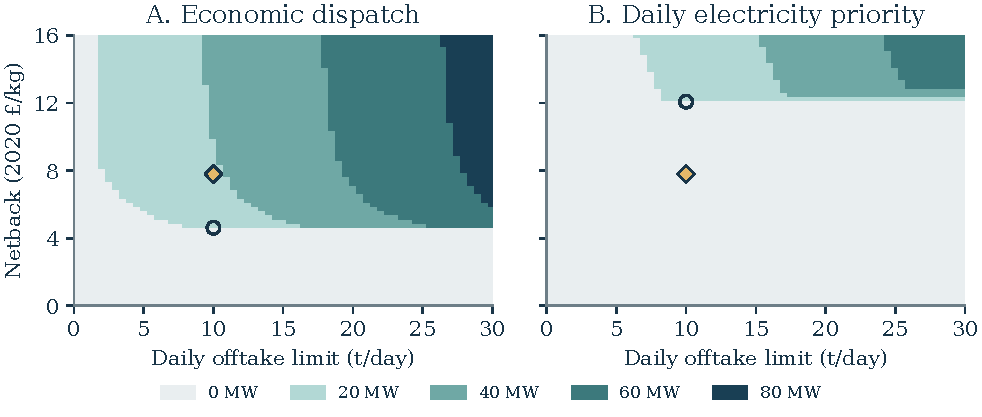
\includegraphics[width=\linewidth]{figures/contract-trigger.pdf}
  \caption{2023 optimal capacity over the contract grid. Diamonds show the
  reference terms. Open circles show the fixed 20~MW break-even at 10~t/day.}
  \label{fig:contract}
\end{figure}

An annual floor lets the operator choose which days to preserve sales.
Table~\ref{tab:sales-floor} compares floors against the 215.1~TWh sold
under A without investment. The 99.99\% floor binds in this case.

\begin{table}[H]
  \centering\small
  \caption{Annual sales floors in A. The first row shows unrestricted sales.
    The lost sales column reports realised reductions.}
  \label{tab:sales-floor}
  \begin{tabularx}{\linewidth}{@{}Y r r r r@{}}
    \toprule
    Scenario & Sales retained (\%) & Lost sales (GWh) & \hydrogen{} (MW)
      & Gain (\gbp m/yr) \\
    \midrule
    Unrestricted          & 99.9266 & 157.92 & 20 & 8.57 \\
    Restore half the loss & 99.9633 &  78.96 & 20 & 5.19 \\
    Tight sales floor     & 99.9900 &  21.51 & 20 & 1.04 \\
    Preserve all sales   & 100.0000 &   0.00 &  0 & 0.00 \\
    \bottomrule
  \end{tabularx}
\end{table}

\paragraph{Model checks.}
The 2023 joint Xpress model is optimal (2,556 rows, 1,827 columns).
Checks reconcile flows and revenues in 42 optimal and two rule schedules,
with physical residuals below 0.001~MWh. Xpress confirms eight enumerated
contract points spanning zero to expansion. Independent results match 18
cases \cite{peer}.

\samplebreak
\subsection{Robustness, validation and returns}
The 20~MW capacity is fixed in the 2022--25 replays, with dispatch
reoptimised on each realised year. The site-only case gives background
generation priority and limits device input to the simulated farm.

\begin{table}[H]
  \centering\small
  \caption{Fixed 20~MW replays. Values are gains against the corresponding
    zero-investment case, in \gbp m/year.}
  \label{tab:replay}
  \begin{tabularx}{\linewidth}{@{}Y r r@{}}
    \toprule
    Period and assumptions & A. Economic dispatch & B. Daily electricity priority \\
    \midrule
    2022 & 8.91 & 7.31 \\
    2023 & 8.57 & \negval{1.07} \\
    2024 & 11.95 & \negval{1.00} \\
    2025 & 13.17 & 4.48 \\
    2025, \gbp 4/kg and 5~t/day & \negval{0.24} & \negval{0.77} \\
    2023, wind-site boundary & 8.17 & \negval{1.07} \\
    \bottomrule
  \end{tabularx}
\end{table}

Both policies lose money in the 2025 downside at \gbp 4/kg and 5~t/day.
At 10~t/day, B's 2025 break-even falls to \gbp 3.13/kg as surplus rises.
In 2023, A still gains \gbp 7.29m/year at 25\% higher initial installation
cost and an 8\% real discount rate, with stack cost held fixed. The
strict-quality 2023 sample retains the base capacities.

\paragraph{Storage check.}
A full usable discharge on every positive-price day earns at most
\gbp 48.7k per module in 2023 even with free charging, below the
\gbp 96.4k annual cost. In A with one battery and no electrolyser, replacing the annual
balance with \(s_t=s_{t-1}+\eta c_t-r_t/\eta\),
\(0\le s_t\le E_B b\) and \(s_0=s_{|\mathcal T|}=0\) cuts operating value from
\gbp 13.3k to \gbp 4.3k. This is below the lower fixed-cost case of
\gbp 11.1k/year. Intraday and ancillary value lie outside this daily case.

\paragraph{Cash flow.}
The 2023 A case receives \gbp 23.97m in hydrogen netback per year, forgoes
\gbp 12.39m in power sales and spends \gbp 0.52m on fixed operations.
After \gbp 2.49m/year for capital and stacks, annual gain is \gbp 8.57m.
For \gbp 29.21m paid upfront, payback is 2.64 years simple and 2.90 years
discounted. Repeating 2023 operations for 30 years with renewals in years
11 and 22 and zero residual value gives \gbp 131.78m net present value.


\section{Tier 1 recommendation}
Retain the existing assets while confirming hydrogen acceptance and
delivered netback, site access to electricity and sales obligations.
Consider one 20~MW module if the agreed terms clear the relevant threshold.
Revisit storage when a paid service or a different operating window can
cover its costs.

\begin{thebibliography}{9}
\small
\setlength{\itemsep}{1pt}
\bibitem{brief} MMCS. \emph{2026/27 Project Brief}, pp.~2--3 and 5--6.
\bibitem{repair} MMCS Group 15. \emph{Project data repair, release 20261104-v2}.
  \href{https://github.com/MocryMin/mmcs-group15-project/tree/71ce76e/Tier1/public/data_quality/full_data_repair/20261104-v2}{Data, methods and audit}.
\bibitem{cpi} Office for National Statistics.
  \href{https://www.ons.gov.uk/economy/inflationandpriceindices/timeseries/d7bt/mm23}{Consumer Prices Index, D7BT}.
\bibitem{dea} Danish Energy Agency.
  \href{https://ens.dk/media/6589/download}{Technology data for energy storage},
  worksheet 180 Lithium Ion Battery.
\bibitem{iea} International Energy Agency.
  \href{https://www.iea.org/reports/global-hydrogen-review-2025/executive-summary}{\emph{Global Hydrogen Review 2025}}, electrolyser investment costs.
\bibitem{beis} Department for Business, Energy and Industrial Strategy.
  \href{https://assets.publishing.service.gov.uk/media/611b710e8fa8f53dc994e59d/Hydrogen_Production_Costs_2021.pdf}{\emph{Hydrogen Production Costs 2021}}
  and technical assumptions annex.
\bibitem{har} Department for Energy Security and Net Zero.
  \href{https://www.gov.uk/government/publications/hydrogen-production-business-model-net-zero-hydrogen-fund-shortlisted-projects/hydrogen-production-business-model-net-zero-hydrogen-fund-har1-successful-projects}{\emph{Hydrogen Allocation Round 1 successful projects}}, 2023.
\bibitem{basis} MMCS Group 15.
  \href{https://github.com/MocryMin/mmcs-group15-project/blob/38f82d5/Tier1/public/research_1103/controller/mocry-codex/20261103-v1.1/R4-finance-data/REPORT.md}{\emph{Financial conversions and technology cost basis}}, R4, 2026.
\bibitem{peer} Clever User.
  \href{https://github.com/MocryMin/mmcs-group15-project/tree/024edd1/Tier1/workspaces/mocry/cleveruser/tier1/20261105-v1}{\emph{Independent Tier 1 implementation}},
  20261105-v1, commit \texttt{024edd1}.
\end{thebibliography}

\end{document}
